		\paragraph{QuizziPedia::Front-End::Directives::SortImagesAnswerDirective}
		
		\label{QuizziPedia::Front-End::Directives::SortImagesAnswerDirective}
		
		\begin{figure}[ht]
			\centering
			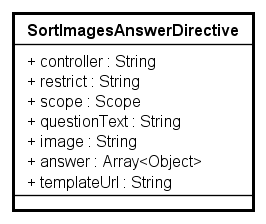
\includegraphics[scale=0.80,keepaspectratio]{UML/Classi/Front-End/QuizziPedia_Front-end_Templates_SortImagesAnswerTemplate.png}
			\caption{QuizziPedia::Front-End::Directives::SortImagesAnswerDirective}
		\end{figure} \FloatBarrier
		
		\begin{itemize}
			\item \textbf{Descrizione}: rappresenta il componente grafico che permette all'utente di visualizzare la domanda ad ordinamento di immagini. Viene visualizzato dinamicamente all'interno delle views \texttt{TrainingView} e \texttt{FillingQuestionnaireView} mediante il \textit{controller\ped{G}} \\ \texttt{QuestionsController};
			\item \textbf{Utilizzo}: viene utilizzato per consentire all'utente la compilazione della domanda ad ordinamento di immagini;
			\item \textbf{Relazioni con altre classi}: 
			\begin{itemize}
				\item \textbf{IN \texttt{QuestionsModelView}}: classe di tipo \textit{modelview\ped{G}} la cui istanziazione è contenuta all'interno della variabile di ambiente \$scope di \textit{Angular\ped{G}}. All'interno di essa sono presenti le variabili e i metodi necessari per il \textit{Two-Way Data-Binding\ped{G}} tra le directive che compongono dinamicamente la vista della domanda e il \textit{controller\ped{G}} \texttt{QuestionsController};
				\item \textbf{OUT \texttt{TrainingView}}: \textit{view\ped{G}} principale della modalità allenamento. Conterrà i vari templates di ogni domanda dell'allenamento;
				\item \textbf{OUT \texttt{FillingQuestionnaireView}}: \textit{view\ped{G}} principale per la compilazione del questionario; conterrà i vari templates di ogni domanda appartenente al questionario;   
				\item \textbf{IN \texttt{LangModel}}: rappresenta il modello delle informazioni per la giusta traduzione dell'applicazione.
			\end{itemize}
			\item \textbf{Attributi}: 
			\begin{itemize}
				\item \texttt{+ questionText: String} \\ Identifica il testo della domanda;
				\item \texttt{+ image: String} \\ Identifica l'url di una possibile immagine nella domanda;
				\item \texttt{+ answers: Array<Object>} \\ Array che contiene coppie di valori. Queste coppie sono formate da:
				\begin{itemize}
					\item \texttt{+ type: String} \\ Indica la tipologia della risposta;
					\item \texttt{+ text: String} \\ Contiene il testo dell'affermazione;
					\item \texttt{+ url: String} \\ Rappresenta l'immagine della risposta;
					\item \texttt{+ attributesForSorting: Mixed} \\ Contiene i seguenti attributi:
					\begin{enumerate}
						\item \texttt{+ position: Boolean} \\ Contiene la giusta posizione del testo o dell'immagine nell'esercizio di ordinamento.
					\end{enumerate}
				\end{itemize}
				\item \texttt{+ controller: String} \\ Stringa contenente il nome del \textit{controller\ped{G}} della direttiva;
				\item \texttt{+ restrict: String} \\ Stringa che permette di definire le modalità di inserimento della direttiva all'interno della pagina;
				\item \texttt{+ scope: Scope} \\Oggetto \texttt{\$scope} interno della direttiva, contiene le funzionalità per gestire i dati presenti all'interno;
				\item \texttt{+ templateUrl: String} \\ Stringa contenente il percorso del file \textit{HTML\ped{G}} che contiene la direttive.
			\end{itemize}
		\end{itemize}
		